a) Escribir un programa que realice una búsqueda
secuencial en una lista lineal vinculada en la
que se puedan ingresar y eliminar datos. Debe incluir
las mejoras de mover al frente y transposición, si un
elemento se ha buscado más de tres veces, se aplica
mover al frente, de lo contrario se aplica transposición.
\lstinputlisting{Busqueda/TareaA.c}
Capturas de Pantalla de Busqueda/TareaA.c
\newline
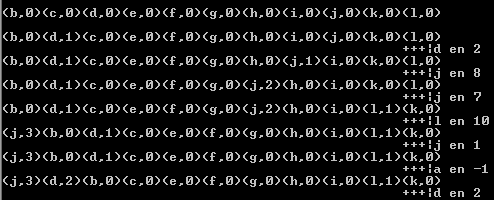
\includegraphics{Busqueda/img/TareaA_1.png}
